% CS 549 Project Final Report
% Financial Transaction Category Classification Using Machine Learning Models
%
% NeurIPS-style formatting (per CS549_spring26_course_projects.pdf rubric).
% To use the official NeurIPS template, drop neurips_2024.sty next to this
% file and replace the documentclass + style line with:
%   \documentclass{article}
%   \usepackage[final]{neurips_2024}
% The article-class fallback below produces a comparable layout without
% requiring the external style file.

\documentclass[11pt]{article}

\usepackage[letterpaper, margin=1in]{geometry}
\usepackage[utf8]{inputenc}
\usepackage[T1]{fontenc}
\usepackage{mathptmx}  % Times New Roman text + math (per rubric formatting)
\usepackage[scaled=0.85]{beramono}  % Heavier monospace that pairs with Times
\usepackage{microtype}
\usepackage{graphicx}
\usepackage{booktabs}
\usepackage{array}
\usepackage{enumitem}
\usepackage{hyperref}
\usepackage{xcolor}
\usepackage{amsmath, amssymb}
\usepackage{caption}
\usepackage{subcaption}
\usepackage{titlesec}
\usepackage{float}
\usepackage{placeins}

% Allow floats to occupy more of a page so they don't get deferred.
\renewcommand{\topfraction}{0.9}
\renewcommand{\bottomfraction}{0.8}
\renewcommand{\textfraction}{0.07}
\renewcommand{\floatpagefraction}{0.7}

\hypersetup{
    colorlinks=true,
    linkcolor=black,
    citecolor=black,
    urlcolor=blue,
}

% Section spacing closer to NeurIPS look.
\titleformat{\section}{\normalfont\large\bfseries}{\thesection}{1em}{}
\titleformat{\subsection}{\normalfont\normalsize\bfseries}{\thesubsection}{1em}{}

\begin{document}

\begin{center}
{\LARGE\bfseries Financial Transaction Category Classification \\[0.25em]
Using Machine Learning Models \par}

\vspace{1.8em}

{\large Dariel Gutierrez \quad Bradley Mustoe \quad Joshua Sherrod \quad Zander Barajas \par}

\vspace{1em}

{\normalsize CS 549 Machine Learning \\
Professor Joanne Chen \\
May 8, 2026 \par}
\end{center}

\vspace{2em}

\begin{center}
{\large\bfseries Abstract}
\end{center}
\vspace{-0.5em}

\noindent
We classify personal financial transactions into spending categories
using their amount, description, merchant, and date. Four classical
supervised models (Logistic Regression, SVM, Random Forest, and a
multilayer perceptron) are trained on two merged Kaggle datasets
totaling roughly $12{,}000$ labeled transactions across $18$
categories. Every model uses the same feature representation: a TF-IDF
vectorizer over descriptions, one-hot encodings of the categorical
fields, and a standardized amount column. Each is tuned with
cross-validation or a validation-set grid, then refit on the combined
training and validation data before a final test evaluation. On the
baseline dataset, Random Forest reaches the best macro F1 ($0.162$)
and the Neural Network the best accuracy ($0.177$), but every model
lands within $0.08$ macro F1 of the others regardless of which
architecture we choose. When we re-run the pipeline across four
data-quality variants of the dataset, performance jumps from the
$0.09$--$0.20$ range up into the $0.80$--$1.00$ range once we strip
out the synthetic Faker-generated descriptions in one source and the
noisy labels in the other. Data quality, not model choice, is what
limits this task.

\newpage

\section{Introduction}

Financial transaction category classification is an important task in
financial management systems because it enables automated budgeting,
expense tracking, and fraud monitoring. Many banking apps rely on machine
learning to sort user transactions into spending groups, which saves
users from organizing their finances by hand. The goal of this project
was to design, implement, and compare supervised machine learning models
that classify financial transactions into the correct category.

The datasets used in this project contain both structured and unstructured
financial data. Structured features include transaction amount, payment type,
account name, user identifier, and transaction date. Unstructured features
include merchant names and transaction descriptions. These text-based fields
often contain clues about the category. For example, a restaurant name
suggests a dining transaction, while a utility provider name suggests a
recurring bill. We picked these datasets because they contain realistic
transaction records with multiple spending categories and a mix of
numerical and textual fields. Since the
datasets originated from different sources, preprocessing and schema
alignment were necessary before training. The preprocessing pipeline
standardized category labels, removed duplicate records, handled missing
values, normalized text formatting, and merged the datasets into a unified
dataset containing 12{,}283 transactions across 18 categories.

Feature extraction was a key step. To turn textual transaction
descriptions into numerical inputs, we used TF-IDF vectorization. TF-IDF was selected because it captures the
importance of words within transaction descriptions while reducing the
influence of common words that appear across many transactions. In addition,
categorical variables were encoded using one-hot encoding, and transaction
amount features were standardized to improve compatibility with machine
learning algorithms.

\section{Related Work}

Recent related work uses transformer-based architectures to better model
the noisy text descriptors that come with financial transactions. The paper
``Hierarchical Classification of Financial Transactions Through Context-Fusion
of Transformer-based Embeddings and Taxonomy-aware Attention Layer''
\cite{busson2023hierarchical} proposes Two-headed DragoNet, a model that uses
stacked Transformer encoder layers to produce contextual embeddings from
merchant name and business activity. These embeddings are fused and fed into
two output heads that together predict transaction categories under a
hierarchical structure. The authors introduce a taxonomy-aware attention
layer to enforce consistency with the predefined category hierarchy, and they
report F1-scores around 93--95\%.

Our project follows the same general direction but takes a simpler,
consumer-oriented approach. Like the Two-headed DragoNet paper, we
aim to predict semantic categories of financial transactions based primarily
on textual descriptors and structured fields, and we evaluate model
performance with classification metrics such as accuracy, precision, recall,
and F1-score. However, instead of designing a specialized hierarchical
Transformer architecture, we concentrate on classical supervised machine
learning classification models.

\section{Methodology}

\subsection{Data Preprocessing}

The preprocessing pipeline was designed to combine two separate financial
transaction datasets~\cite{kaggle_d1, kaggle_d2} into one consistent
supervised learning dataset. Since the datasets used different column names
and slightly different category formats, the first step was schema
standardization. The project defined a
shared set of canonical columns: \texttt{date}, \texttt{description},
\texttt{amount}, \texttt{transaction\_type}, \texttt{account\_name},
\texttt{category}, and \texttt{source\_dataset}. Each raw dataset was loaded
separately, renamed into this shared schema, and tagged with a
\texttt{source\_dataset} field so the source of each row could still be
tracked after merging. The two datasets were then cleaned and standardized.

Transaction descriptions were converted into normalized text by stripping
whitespace, converting text to lowercase, removing non-alphanumeric
characters, collapsing repeated whitespace, and storing the result as
\texttt{description\_clean}. Transaction amounts were converted into numeric
values, and rows with invalid or missing amounts were removed. Dates were
parsed into datetime format, and rows with invalid dates were also removed.
Category labels were normalized to reduce mismatches between the two
datasets.

Similar labels were mapped into shared category names. For example,
"restaurants", "fast food", "food \& dining", "coffee shops", and
"food \& drink" were merged into Dining; "movies \& dvds", "television",
and "music" were merged into Entertainment; "salary" and "paycheck" were
merged into Income; and labels such as "rent", "utilities", "internet",
and "mobile phone" were merged into broader standardized categories where
appropriate.

After both datasets were standardized, they were merged into a single
dataframe. Duplicate transactions were removed using the fields
\texttt{date}, \texttt{description\_clean}, \texttt{amount}, and
\texttt{category}, which reduced repeated examples that could bias model
training. The final combined dataset was sorted by date and cleaned
description.

\subsection{Feature Engineering}

The preprocessing script then created train, validation, and test splits
using stratified sampling, so each split keeps the same class
proportions as the full dataset. The test set used 20\% of the data, and the remaining data was
split again into training and validation sets (resulting in a 64/16/20
train/val/test split). Feature engineering was handled through a shared
feature transformer used across all models. The cleaned transaction
description, \texttt{description\_clean}, was transformed using TF-IDF
vectorization with up to 10{,}000 features, 1-to-4 word n-grams,
\texttt{min\_df}=2, \texttt{max\_df}=0.95, and sublinear term-frequency
scaling. Categorical features, including \texttt{date\_month},
\texttt{date\_day\_of\_week}, \texttt{transaction\_type}, and
\texttt{account\_name}, were encoded using one-hot encoding with
unknown-value handling enabled. The numerical amount feature was
standardized using \texttt{StandardScaler} so that models sensitive to
feature scale would not be skewed by the raw dollar amounts. These
transformations were combined using a single \texttt{ColumnTransformer},
ensuring that all models were trained on the same feature representation.

\subsection{Model Selection}

\paragraph{Logistic Regression (Joshua Sherrod).}
Logistic Regression was selected as a baseline model for this project because
it is simple, efficient, and widely used for classification tasks. It can
model the probability of a transaction belonging to a specific category,
which makes it a strong option for multi-class classification problems and a
useful linear baseline against which the other three models can be compared.

\paragraph{Random Forest (Bradley Mustoe).}
Random Forest was selected for this project because it is an ensemble
learning method that combines multiple decision trees to improve
classification accuracy and reduce overfitting. Tree ensembles handle
mixed numerical/categorical inputs without additional encoding effort and
are well suited to a TF-IDF + one-hot feature matrix that contains many
sparse, weakly-informative columns.

\paragraph{Support Vector Machine (Dariel Gutierrez).}
Since transaction descriptions were represented using TF-IDF vectors, a
linear SVM was appropriate for learning category boundaries from text-heavy
features. Both \texttt{LinearSVC} and an RBF kernel were evaluated, but the
performance difference was small, so \texttt{LinearSVC} was retained for its
significantly lower training cost. The SVM also used balanced class weights
to reduce bias toward majority classes.

\paragraph{Neural Network (Zander Barajas).}
The neural network was chosen because it can learn more complex patterns
that simpler models might miss. Since transactions mix numerical fields
(amount), categorical fields (transaction type, account), and text
(merchant name, description), a neural network can pick up on
relationships between these fields better than a strictly linear model.
We used a multilayer perceptron (\texttt{MLPClassifier}) so that it
trains on the same TF-IDF + one-hot + scaled-amount features as the
other three models, letting us compare them directly.

\subsection{Training Process and Hyperparameter Tuning}

All models used the same preprocessed train, validation, and test data. The
shared feature transformer was fit on the training set and then applied to
the validation and test sets. This prevented information from the validation
or test sets from leaking into the feature extraction process. Preprocessing,
feature engineering, model training, and hyperparameter search were
implemented with scikit-learn~\cite{sklearn} and imbalanced-learn~\cite{imblearn};
data manipulation used NumPy~\cite{numpy} and pandas~\cite{pandas}; all
figures were generated with matplotlib~\cite{matplotlib}.

\paragraph{Logistic Regression.}
Hyperparameter tuning used \texttt{GridSearchCV} over the regularization
strength $C \in \{0.01, 0.1, 1.0, 10.0\}$, scored by macro F1 under stratified
5-fold cross-validation on the training set. Class-balanced weighting was
used throughout to compensate for imbalance, and \texttt{max\_iter} was
raised to 1000 to ensure convergence. The best $C$ was then refit on the
combined training and validation data before final evaluation on the test
set.

\paragraph{Support Vector Machine.}
For SVM, hyperparameter tuning was performed using the validation set. The
linear SVM tested several values of the regularization parameter $C$:
$0.01$, $0.05$, $0.1$, $0.5$, $1.0$, $2.0$, $5.0$, and $10.0$. Each candidate
used balanced class weighting. The best configuration was selected based on
macro F1-score on the validation set. After choosing the best
parameters, the model was retrained on the combined training and
validation data before evaluating on the test set, which gave the final
SVM more labeled data without touching the held-out test set.

\paragraph{Random Forest.}
Random Forest tuning used \texttt{RandomizedSearchCV} with $20$ sampled
configurations and stratified 5-fold cross-validation scored by macro F1.
The search space was:
\begin{itemize}[leftmargin=1.5em, itemsep=0pt, topsep=2pt]
\item \texttt{n\_estimators} $\in \{100, 200, 300, 500\}$,
\item \texttt{max\_depth} $\in \{\text{None}, 10, 20, 30\}$,
\item \texttt{max\_features} $\in \{\text{sqrt}, \text{log2}, 0.3\}$,
\item \texttt{min\_samples\_split} $\in \{2, 5, 10\}$,
\item \texttt{min\_samples\_leaf} $\in \{1, 2, 4\}$,
\item \texttt{class\_weight} $\in \{\text{balanced}, \text{balanced\_subsample}\}$.
\end{itemize}
The best estimator was refit on the training data inside the search.

\paragraph{Neural Network.}
The neural network was wrapped in an \texttt{imblearn} pipeline with three
steps: a sparse-safe \texttt{StandardScaler(with\_mean=False)}, a
capped \texttt{RandomOverSampler} that lifts every class with fewer
than $200$ training samples up to $200$, and an \texttt{MLPClassifier} using
the \texttt{adam} solver, \texttt{max\_iter}=120, and early stopping on a
$10\%$ internal validation hold-out. The capped oversampler addresses class
imbalance during training without producing the memorization artifact that
uncapped oversampling caused for very small classes (where the model
simply learned the duplicated rows). Tuning
used \texttt{RandomizedSearchCV} with $15$ sampled configurations and
stratified 5-fold cross-validation scored by macro F1, over:
\begin{itemize}[leftmargin=1.5em, itemsep=0pt, topsep=2pt]
\item \texttt{hidden\_layer\_sizes} $\in \{(128,), (256,), (256,128), (512,256)\}$,
\item \texttt{learning\_rate\_init} $\in \{10^{-4},\, 5{\times}10^{-4},\, 10^{-3},\, 5{\times}10^{-3}\}$,
\item \texttt{alpha} (L2) $\in \{10^{-4}, 10^{-3}, 10^{-2}\}$.
\end{itemize}
Activation (ReLU) and batch size ($256$) were held constant. The best
configuration was refit on train+val. End-to-end runtime on the full
variant was $308$~s ($304$~s search + $4$~s refit; final refit converged in
$16$ epochs under early stopping).

\section{Results}

\subsection{Overall Model Performance}

After preprocessing and feature extraction, the four selected models were
trained and evaluated on the held-out test dataset. Performance was measured
using accuracy, macro precision, macro recall, macro F1-score, and runtime.
Macro-averaged metrics were emphasized because the dataset contained
imbalanced transaction categories: a few classes (Dining, Credit Card
Payment, Bills \& Utilities) account for most rows, while several minority
classes have fewer than $50$ samples. Plain accuracy would reward a model
that simply predicts the majority class, so we treat \textbf{macro
F1-score} as the headline metric and report accuracy/precision/recall as
secondary signals. Runtime is reported alongside accuracy because, in a real
transaction-categorization product where new transactions arrive
constantly, training and inference cost matter for deployability.

The overall evaluation results are shown in Table~\ref{tab:overall-results}.

\begin{table}[!htbp]
\centering
\caption{Overall test-set performance for each model on the
\texttt{full} (D1+D2) variant. Best values per column in \textbf{bold}.}
\label{tab:overall-results}
\begin{tabular}{lcccc}
\toprule
Model & Accuracy & Precision (macro) & Recall (macro) & F1 (macro) \\
\midrule
Logistic Regression & 0.107          & 0.167          & 0.177          & 0.143          \\
Random Forest       & 0.166          & 0.167          & \textbf{0.184} & \textbf{0.162} \\
SVM                 & 0.130          & 0.167          & 0.177          & 0.157          \\
Neural Network      & \textbf{0.177} & \textbf{0.175} & 0.131          & 0.135          \\
\bottomrule
\end{tabular}
\end{table}

\subsection{Best Performance}

Random Forest achieved the highest macro F1-score ($0.162$) and the highest
macro recall ($0.184$). The Neural Network achieved the highest accuracy
($0.177$) and the highest macro precision ($0.175$), but its lower recall
across minority categories pulled its macro F1 below all three other models.
Because the dataset is imbalanced, macro F1 is the primary headline metric,
and Random Forest is the strongest model under that metric.

\subsection{Per-Category Performance}

Model performance varied significantly across transaction categories.
Categories such as Investment, Other, and Credit Card Payment generally
achieved higher F1-scores because these categories contained stronger
semantic patterns and more distinguishable transaction descriptors.
Per-category F1 is shown in Table~\ref{tab:per-category}; categories that
dominate spend volume (Dining, Groceries, Bills \& Utilities) cluster in
the $0.1$--$0.2$ band for every model, while a handful of
distinctive-merchant categories like Investment and Other lift well above
the average.

\begin{table}[!htbp]
\centering
\caption{Per-category F1-score by model on the \texttt{full} variant.}
\label{tab:per-category}
\small
\begin{tabular}{lcccc}
\toprule
Category & LR & RF & SVM & NN \\
\midrule
Alcohol \& Bars         & 0.079 & 0.094 & 0.081 & 0.000 \\
Auto Insurance          & 0.040 & 0.098 & 0.030 & 0.024 \\
Bills \& Utilities      & 0.124 & 0.166 & 0.151 & 0.178 \\
Credit Card Payment     & 0.151 & 0.215 & 0.193 & 0.242 \\
Dining                  & 0.073 & 0.200 & 0.131 & 0.197 \\
Electronics \& Software & 0.029 & 0.000 & 0.027 & 0.000 \\
Entertainment           & 0.124 & 0.127 & 0.116 & 0.110 \\
Gas \& Fuel             & 0.099 & 0.118 & 0.111 & 0.086 \\
Groceries               & 0.125 & 0.183 & 0.143 & 0.170 \\
Haircut                 & 0.032 & 0.044 & 0.044 & 0.000 \\
Health \& Fitness       & 0.127 & 0.182 & 0.098 & 0.118 \\
Home Improvement        & 0.128 & 0.096 & 0.117 & 0.021 \\
Income                  & 0.149 & 0.168 & 0.158 & 0.188 \\
Investment              & 0.481 & 0.508 & 0.536 & 0.400 \\
Mortgage \& Rent        & 0.095 & 0.087 & 0.102 & 0.153 \\
Other                   & 0.500 & 0.431 & 0.519 & 0.400 \\
Shopping                & 0.062 & 0.093 & 0.073 & 0.094 \\
Travel                  & 0.148 & 0.111 & 0.204 & 0.042 \\
\bottomrule
\end{tabular}
\end{table}

These results demonstrate that the models struggled most with categories
that share similar purchasing patterns and merchant descriptors, while
categories with distinctive descriptors (Investment, Other, and Travel
for SVM) lift well above the macro average.

\subsection{Runtime Analysis}

Table~\ref{tab:runtime} reports inference time on the full $2{,}457$-row
test set (single CPU thread) and end-to-end training time (search + refit)
for each model on the \texttt{full} variant. Inference is sub-$25$~ms for
every model, so it is not a discriminator at this scale. Training cost is
dominated by the hyperparameter-search budget. SVM is the clear outlier
on the fast end (under $10$~s) because it skips cross-validation and
\texttt{LinearSVC} fits in a fraction of a second on this
$\sim$$10$k-feature input. The other three models all run 5-fold CV and
take several minutes: LR tests $4$ regularization values ($20$ fits +
final refit), RF samples $20$ configurations ($100$ fits), and the NN
samples $15$ configurations ($75$ fits) on top of the imbalance-mitigation
pipeline.

\begin{table}[!htbp]
\centering
\caption{Runtime on the \texttt{full} variant. Training is wall-clock for
search plus final refit; inference is full-test-set prediction on one CPU
thread.}
\label{tab:runtime}
\begin{tabular}{lcc}
\toprule
Model & Inference (s, full test) & Training (s) \\
\midrule
Logistic Regression & 0.002 & $173$ \\
SVM                 & 0.001 & $7$ \\
Random Forest       & 0.021 & $266$ \\
Neural Network      & 0.009 & $308$ ($304$ search + $4$ refit) \\
\bottomrule
\end{tabular}
\end{table}

\subsection{Visualizations and Confusion Matrices}

Confusion matrices were generated for all four models to visualize
classification behavior and category-level prediction errors. The confusion
matrices revealed that the models frequently confused semantically related
categories.

\begin{figure}[!htbp]
\centering
\begin{subfigure}{0.48\textwidth}
\centering
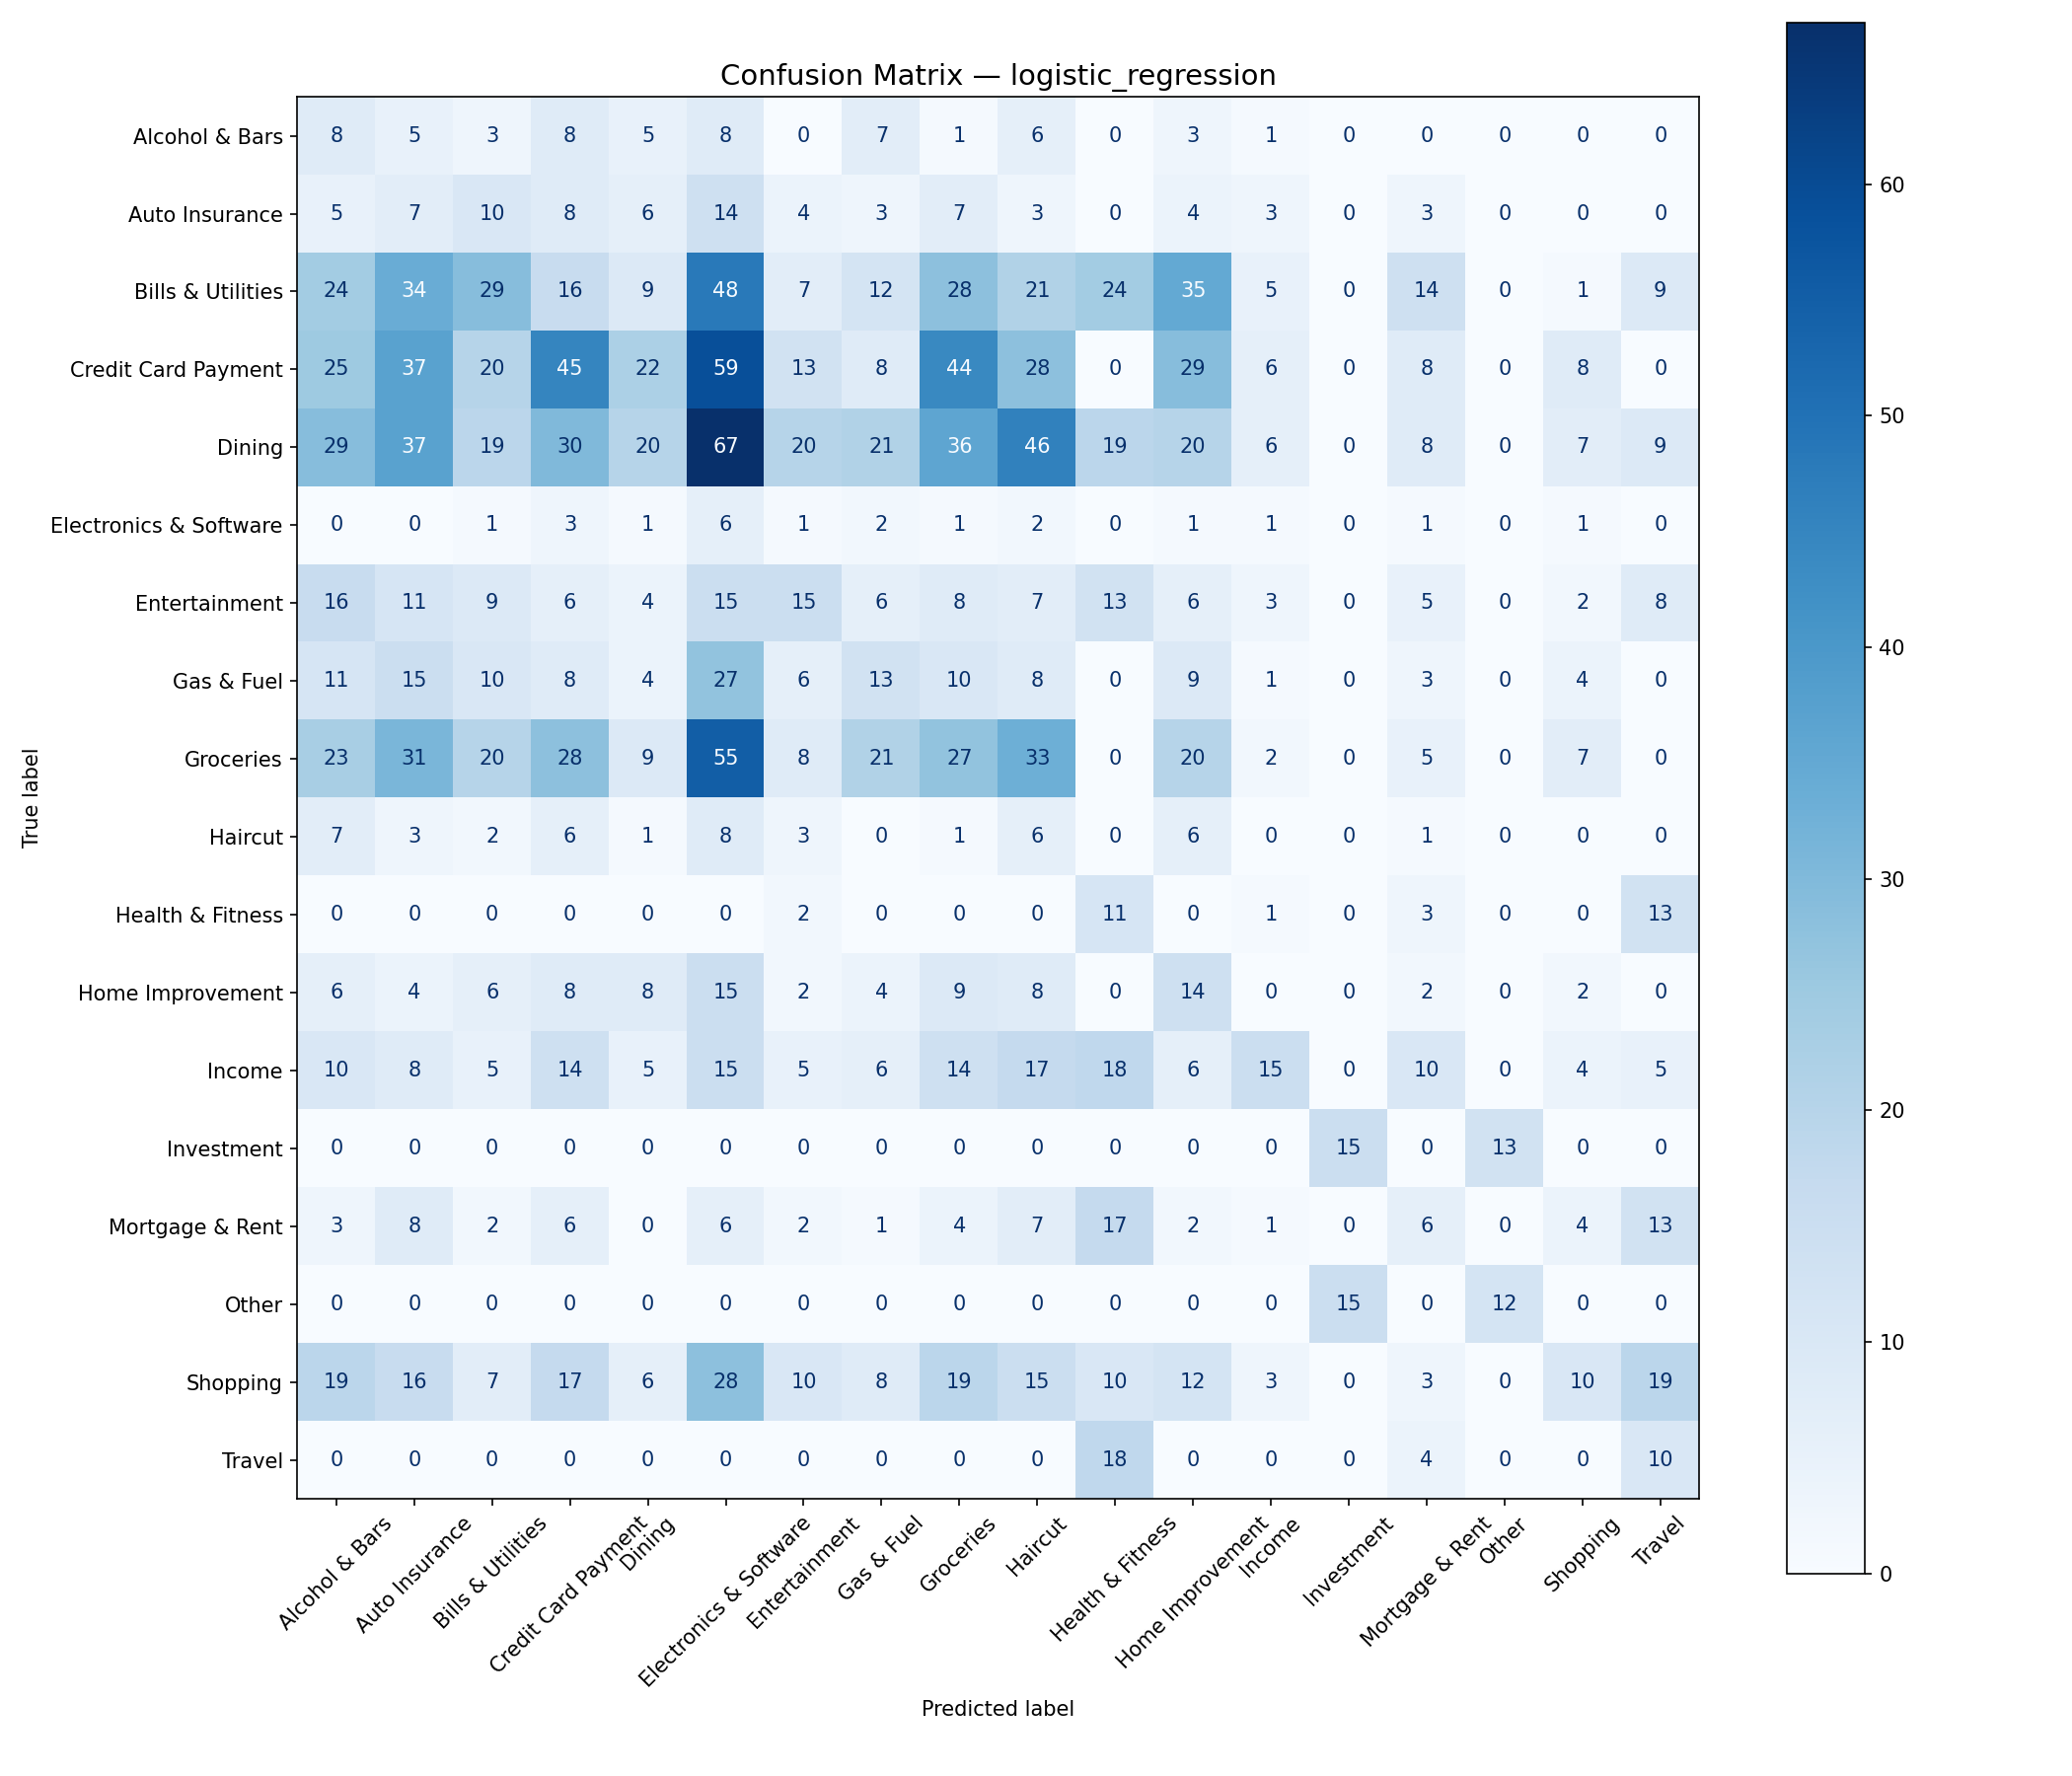
\includegraphics[width=\linewidth]{../models/full/logistic_regression_confusion_matrix.png}
\caption{Logistic Regression}
\end{subfigure}
\hfill
\begin{subfigure}{0.48\textwidth}
\centering
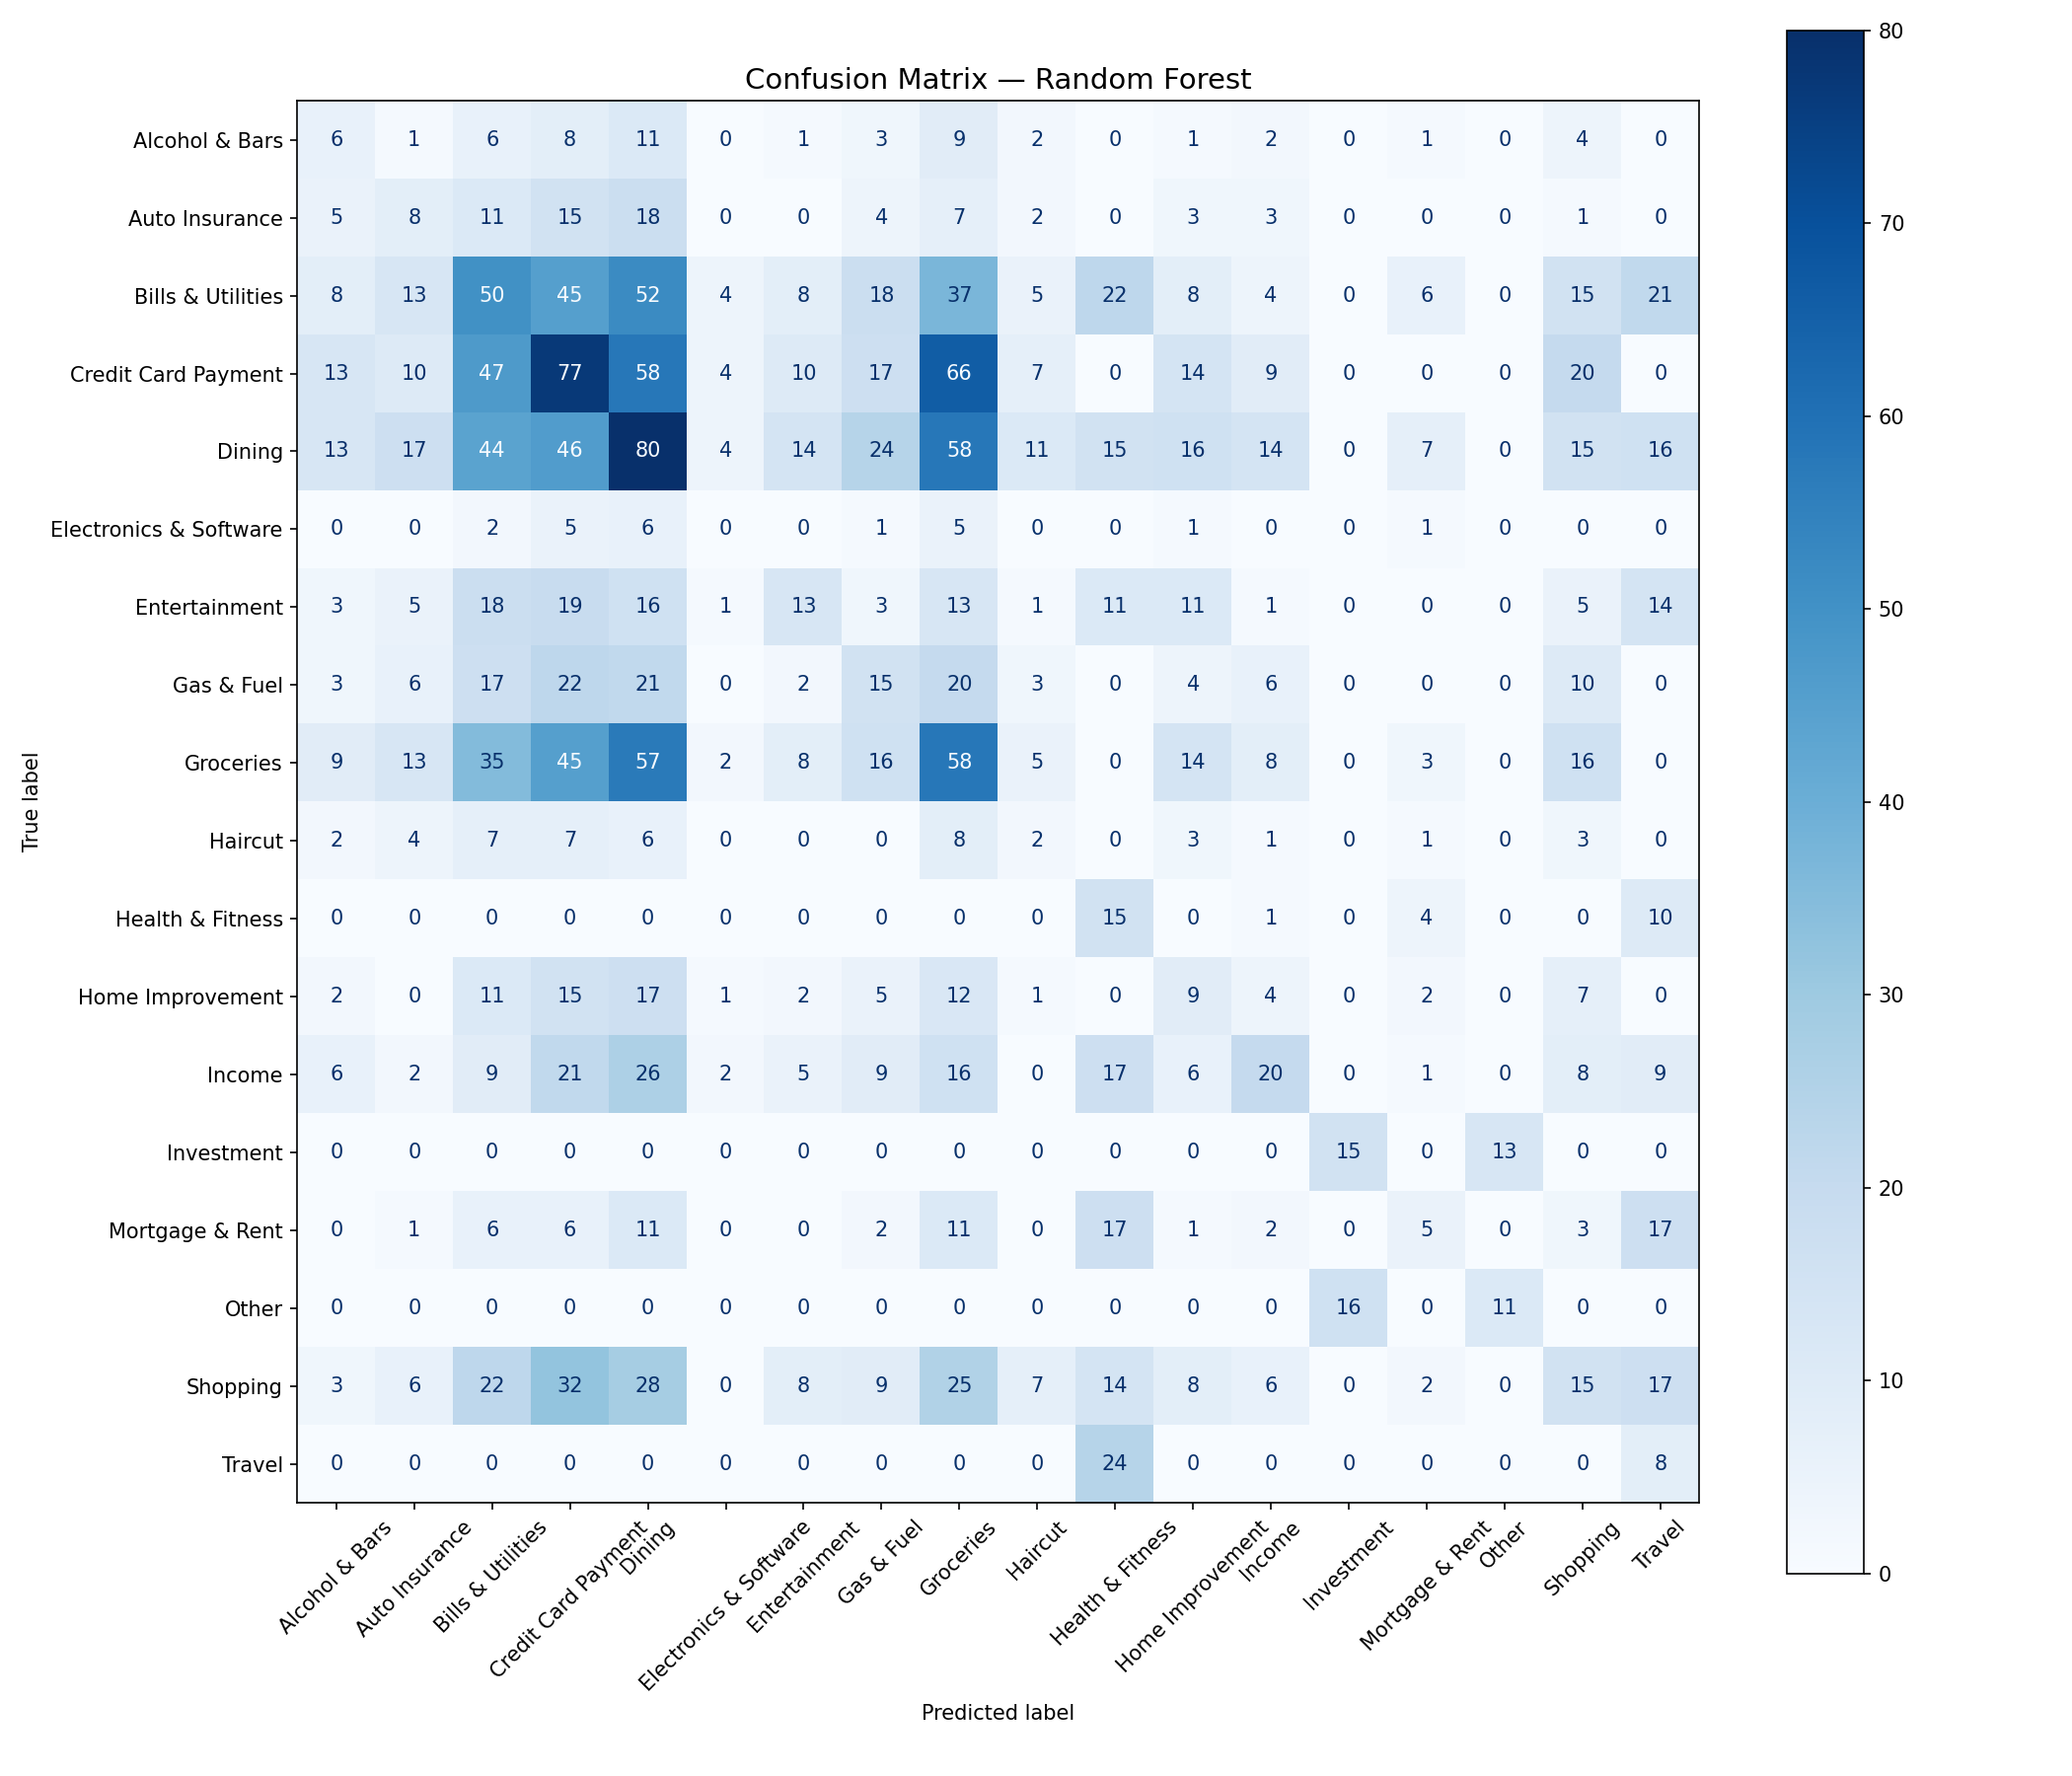
\includegraphics[width=\linewidth]{../models/full/random_forest_confusion_matrix.png}
\caption{Random Forest}
\end{subfigure}

\vspace{0.5em}

\begin{subfigure}{0.48\textwidth}
\centering
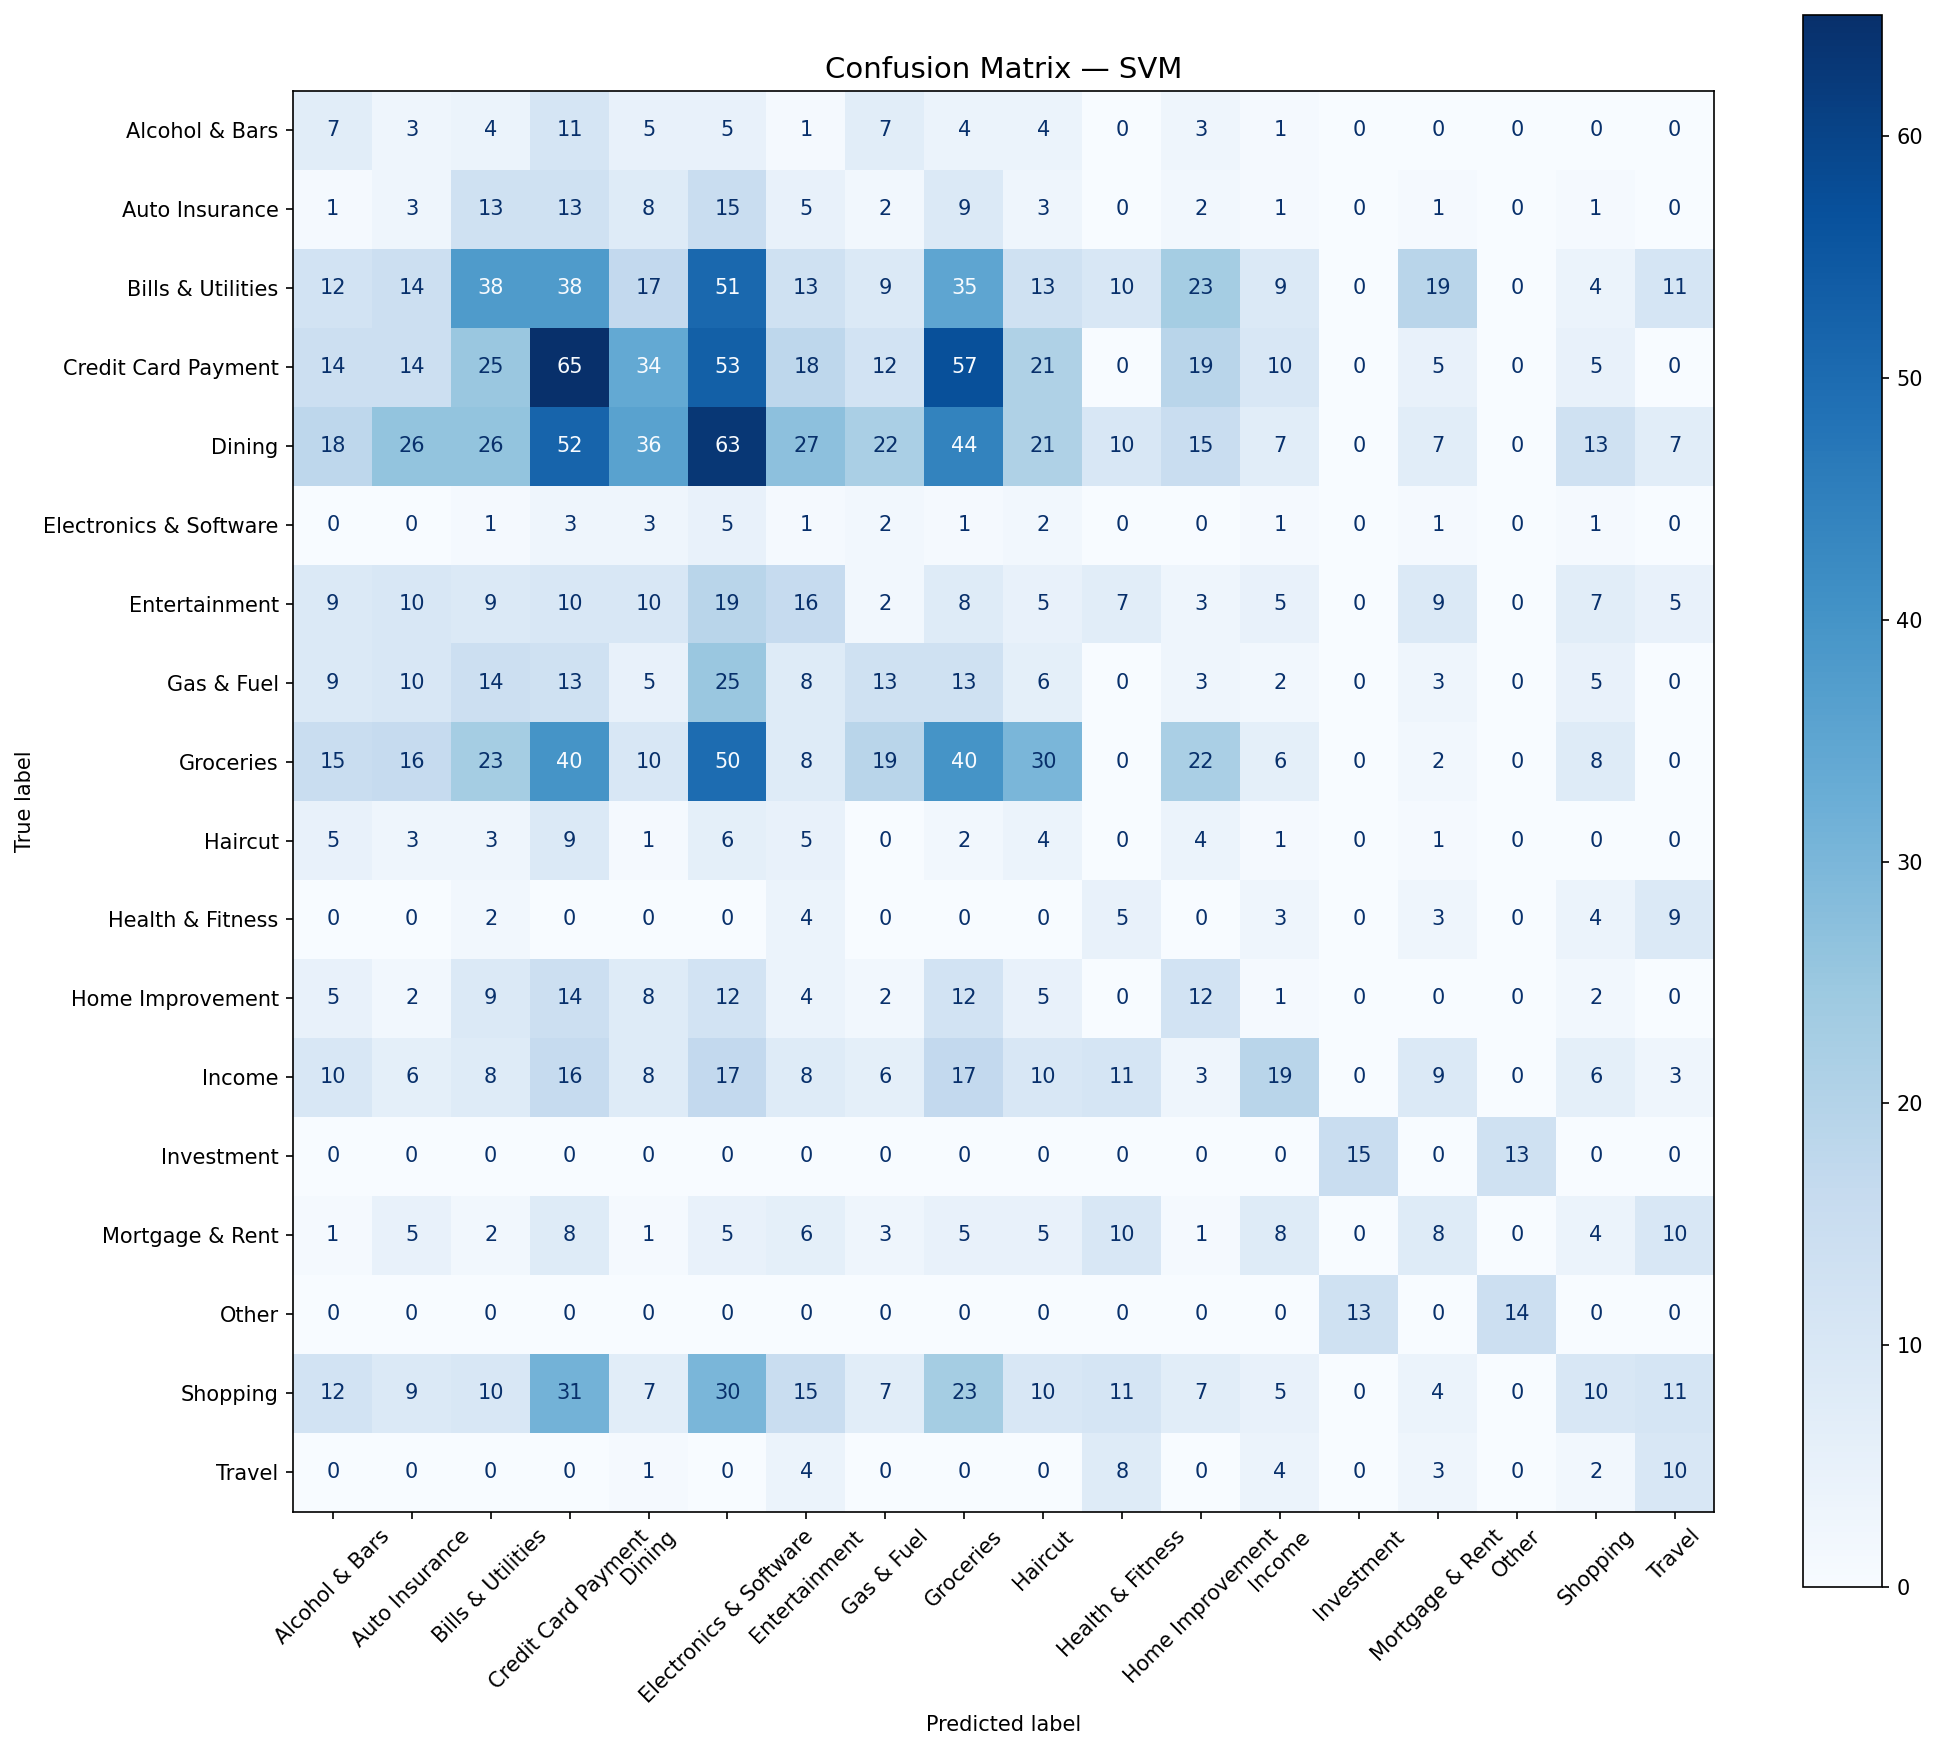
\includegraphics[width=\linewidth]{../models/full/svm_confusion_matrix.png}
\caption{SVM}
\end{subfigure}
\hfill
\begin{subfigure}{0.48\textwidth}
\centering
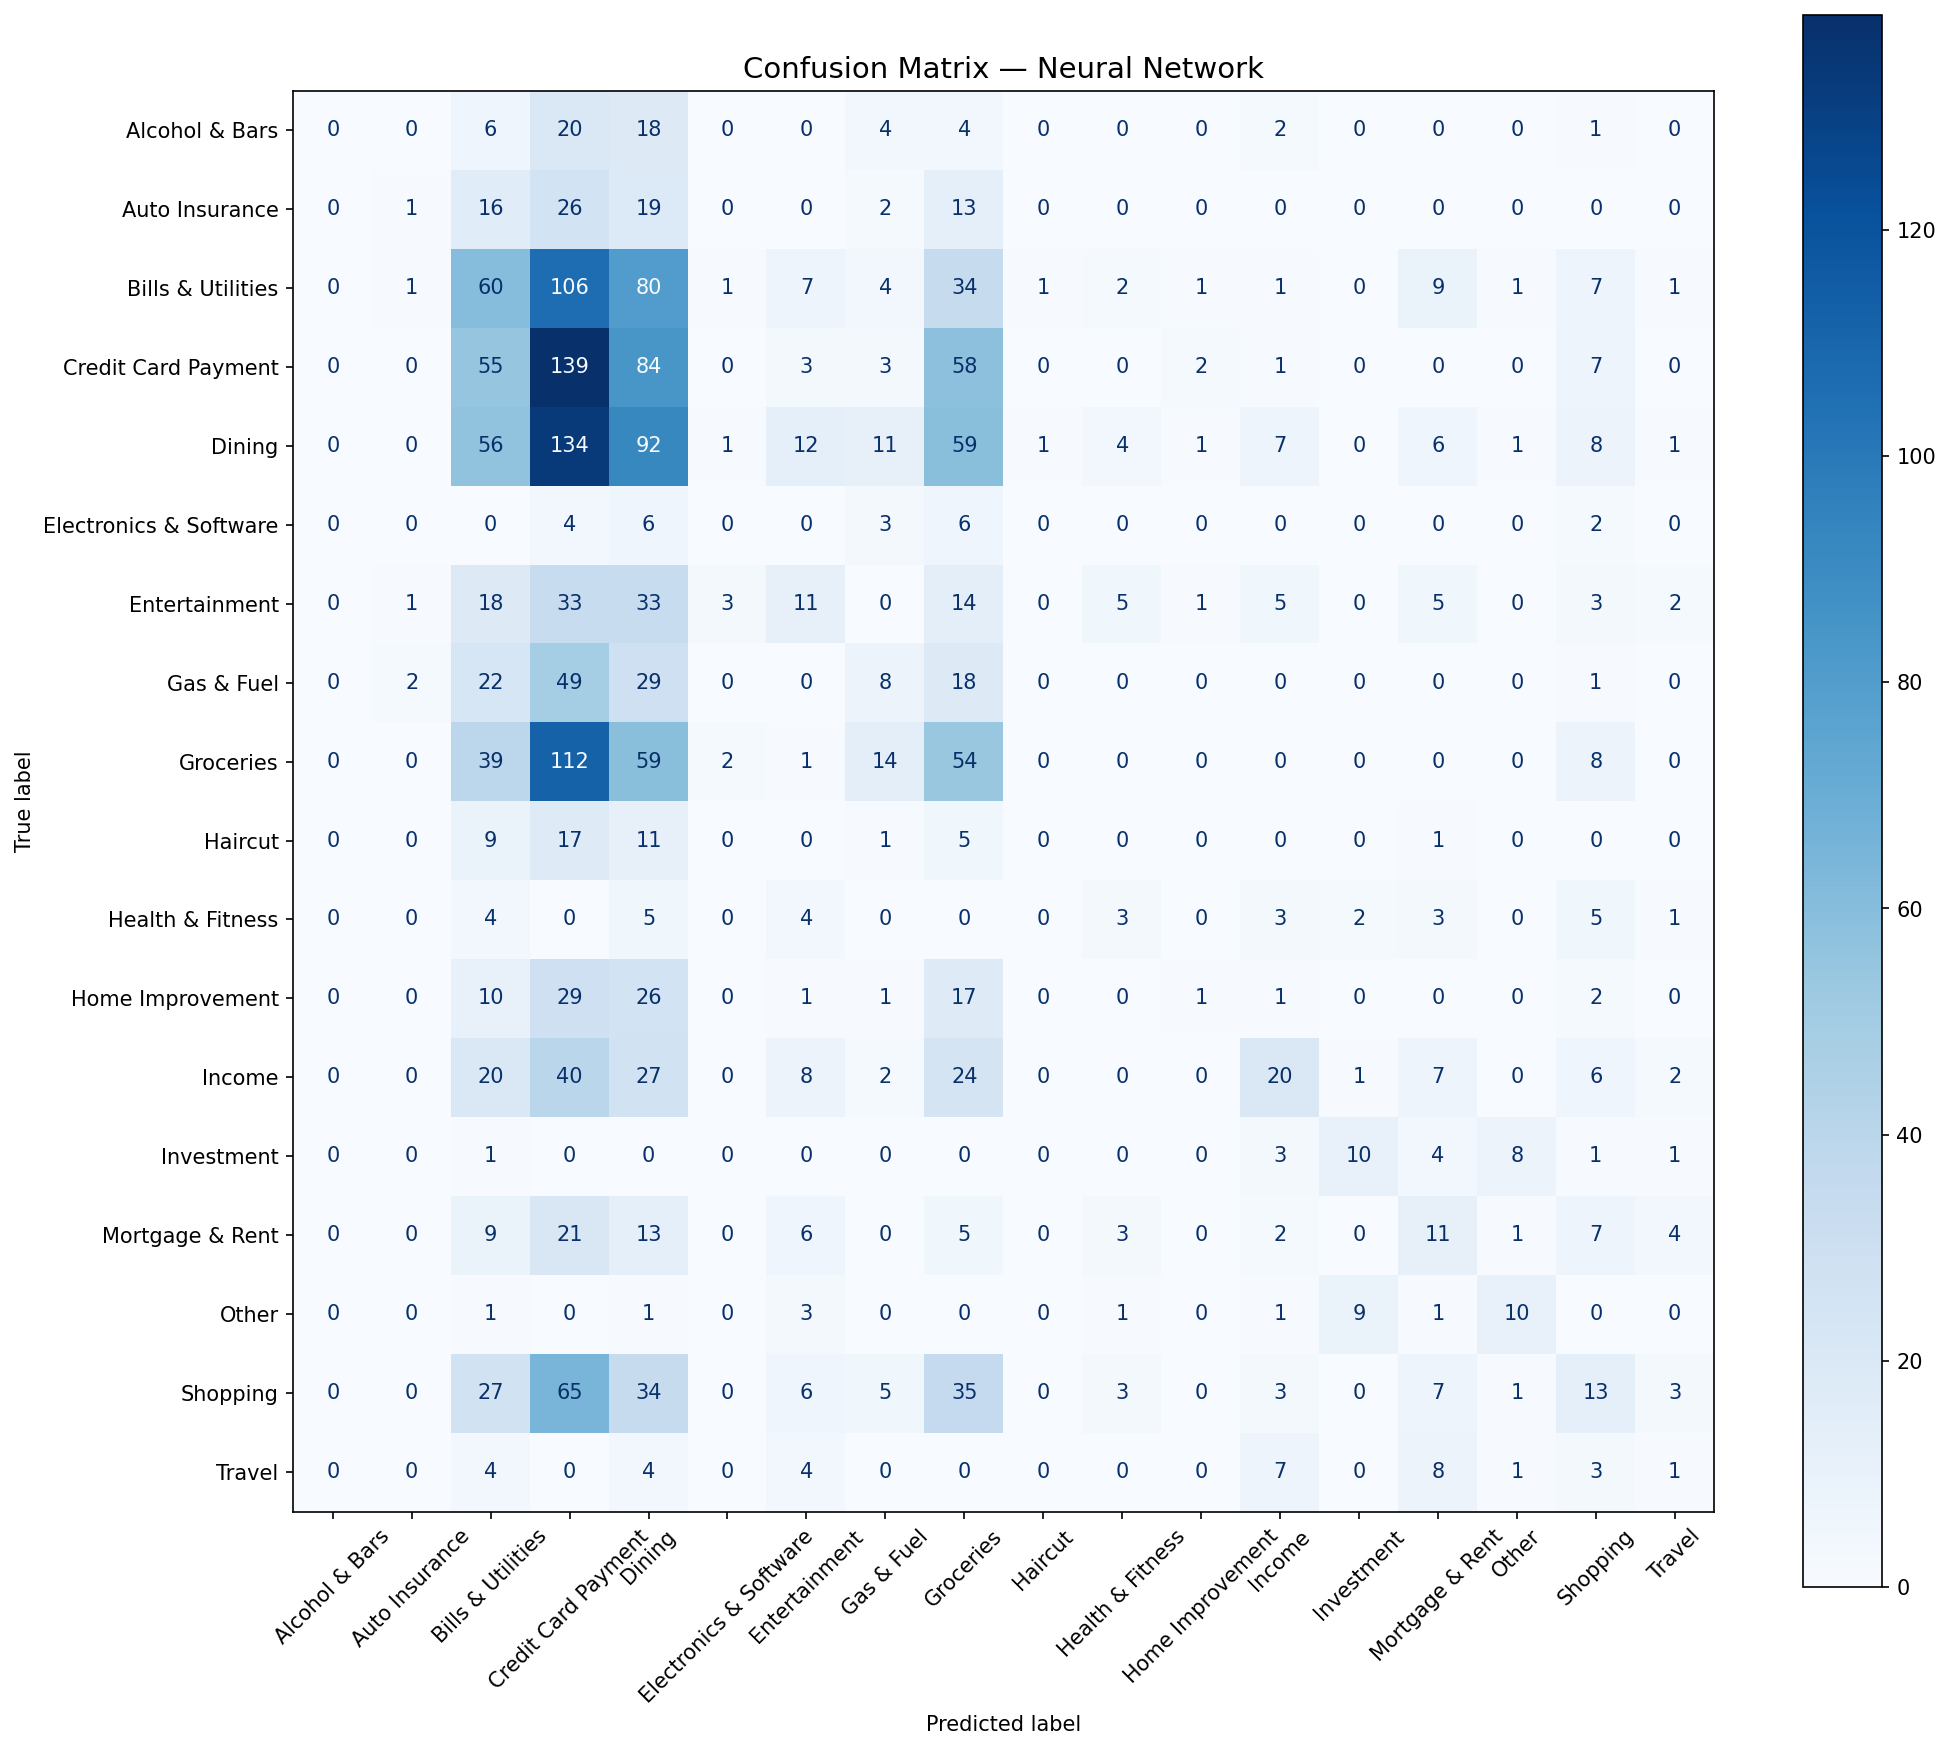
\includegraphics[width=\linewidth]{../models/full/neural_network_confusion_matrix.png}
\caption{Neural Network}
\end{subfigure}
\caption{Confusion matrices for each model on the held-out test set
(\texttt{full} variant).}
\label{fig:confusion-matrices}
\end{figure}

Common misclassification patterns included Dining vs.\ Shopping,
Entertainment vs.\ Travel, and Bills \& Utilities vs.\ Mortgage \& Rent.
These errors suggest that many financial transaction descriptions lack
sufficient contextual information for classical machine learning models to
separate categories cleanly.

The Neural Network's training trajectory is shown in
Figure~\ref{fig:nn-learning-curve}. Training loss decreases monotonically
under the \texttt{adam} optimizer, while the early-stopping holdout
accuracy rises sharply in the first few epochs and then plateaus, which
triggered the early-stopping criterion at epoch $16$ during the final
refit.

\begin{figure}[!htbp]
\centering
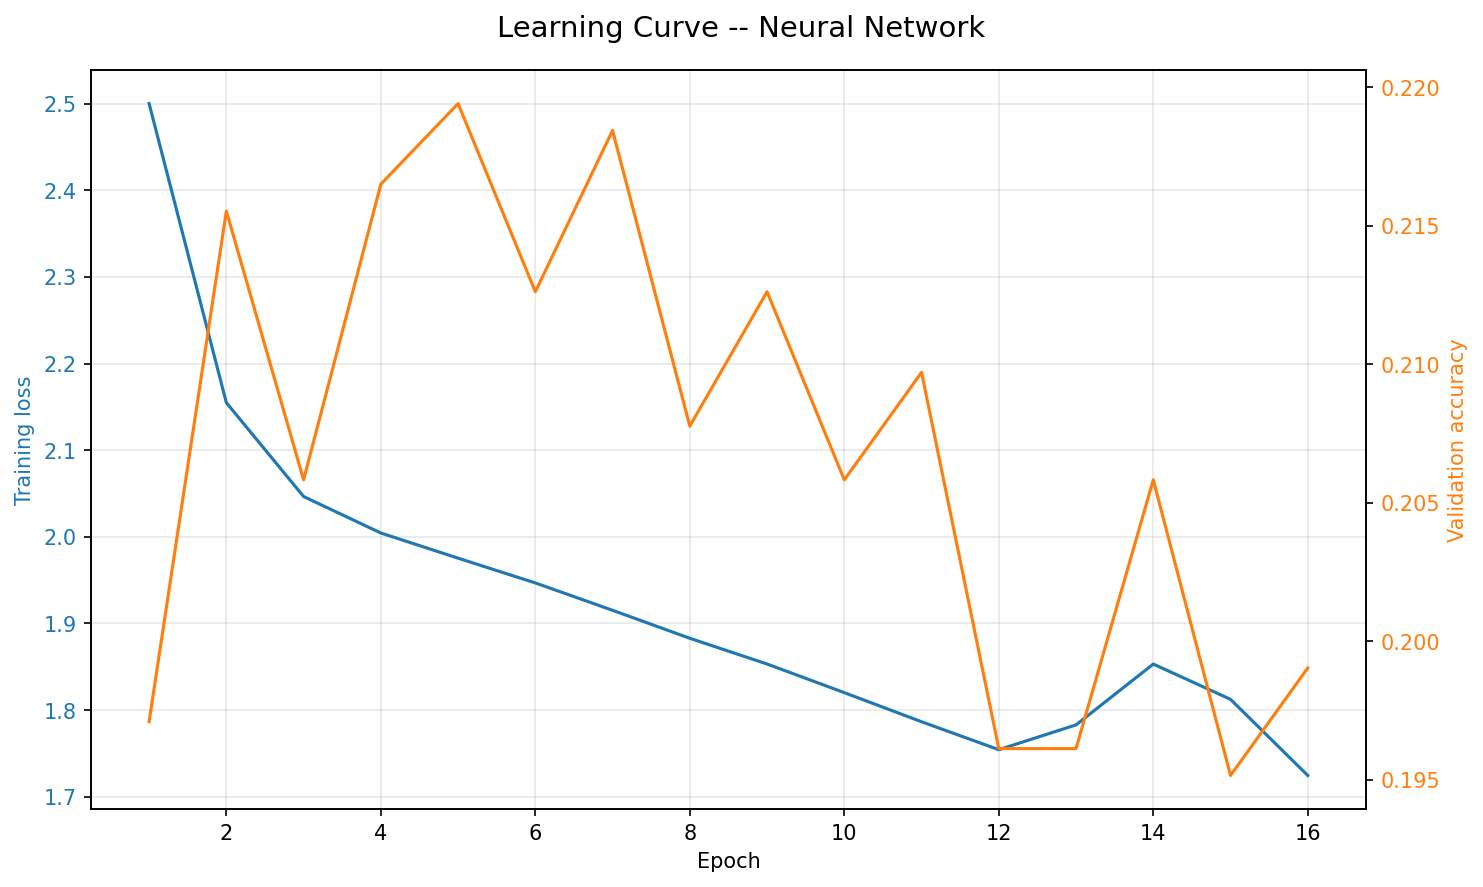
\includegraphics[width=0.7\linewidth]{../models/full/neural_network_learning_curve.png}
\caption{Neural Network learning curve on the \texttt{full} variant:
training loss (left axis) and early-stop validation accuracy (right axis)
versus epoch.}
\label{fig:nn-learning-curve}
\end{figure}

\FloatBarrier
\section{Discussion}

All four models cleared the stratified baseline, but overall metrics
remained modest on the proposal-baseline dataset. The next two
subsections compare model behavior on \texttt{full} and then trace
the ceiling back to data quality through a cross-variant comparison.

\subsection{Comparative Analysis of Models}

\paragraph{Random Forest.}
Random Forest produced the strongest macro F1 ($0.162$) and the highest
macro recall ($0.184$) of any model. The ensemble's variance reduction and
its tolerance of mixed sparse/dense inputs let it pick up signal from both
the TF-IDF text columns and the categorical context features
(\texttt{date\_month}, \texttt{transaction\_type}, \texttt{account\_name}),
which matches our expectation that an ensemble would handle this noisy
feature space better than a purely linear model.

\paragraph{Support Vector Machine.}
The SVM model achieved the second-best macro F1-score ($0.157$). Since the
project relied heavily on TF-IDF text representations, the linear SVM
benefited from working well in high-dimensional sparse feature spaces.
SVM performance was still limited by noisy and overlapping descriptions.
The SVM did produce the highest per-category F1 on Investment ($0.536$),
Other ($0.519$), and Travel ($0.204$), suggesting that a linear SVM
works particularly well on the small set of categories whose
descriptions use distinctive vocabulary.

\paragraph{Neural Network.}
The Neural Network achieved the highest accuracy ($0.177$) and the highest
macro precision ($0.175$) but the lowest macro F1 ($0.135$). The capped
oversampler raised minority training counts to a floor of $200$ rather than
fully balancing every class, which protected the model from
duplication-driven memorization but did not produce a fully calibrated
minority-class recall: macro recall fell to $0.131$, well below the other
three models. In effect the MLP learned to predict majority categories
confidently and skipped many minority predictions altogether (the per-class
table shows zero F1 on Alcohol \& Bars, Electronics \& Software, and
Haircut). On the \texttt{d1} variant the NN sat at the stratified
baseline ($0.123$) while the shallow models climbed to $0.16$--$0.20$
by overfitting chance word-frequency drift -- evidence that the NN's L2
regularization and early stopping correctly refused to learn from
Faker-generated noise rather than memorizing it. End-to-end runtime
was $308$~s, dominated by the $304$~s randomized cross-validation search;
final refit converged in $16$ epochs under early stopping.

\paragraph{Logistic Regression.}
Logistic Regression served as an interpretable baseline. It posted the
weakest overall macro F1 ($0.143$), but still well above the random
baseline, showing that some category structure exists in the feature
space. Its lower performance suggests that this task probably needs the
nonlinear decision boundaries that a purely linear model cannot draw.

\subsection{Cross-Variant Data-Quality Comparison}
\label{sec:ablation}

The proposal-baseline dataset (\texttt{full}) combines two raw Kaggle
sources with very different failure modes.

\textbf{D1 (Personal Finance Dataset)} has clean category labels but
synthetic transaction descriptions. A closer look at the $1{,}500$
descriptions turns up six signals consistent with Python's
\texttt{faker.sentence()} output: $100\%$ of descriptions are unique,
$100\%$ terminate with a period, mean word count is $3.5$ (std $1.0$),
per-category mean character length clusters at $22$--$25$ with within-class
standard deviation of $\sim$$7$, the most frequent tokens are generic
English (\texttt{ahead}, \texttt{son}, \texttt{animal}, \texttt{bad},
\texttt{red}, \texttt{draw}), and per-category top tokens share no overlap
with financial vocabulary.

\textbf{D2 (Personal Transactions UserID)} has real merchant text but
noisy labels introduced by an upstream data-augmentation step. For each
unique \texttt{description\_clean}
we computed the modal-category share -- the fraction of rows of that
description that share its single most-frequent category. The weighted
mean modal share across D2 is $18.1\%$, meaning roughly $82\%$ of D2 rows
are labeled with a category that disagrees with their description's modal
label. The most common description, \texttt{Credit Card Payment},
appears $1{,}848$ times spread across $22$ categories with only $23.4\%$
modal share. To isolate the contribution of each failure
mode, we re-ran the entire pipeline (preprocessing, training, tuning,
evaluation) on four dataset variants:

\begin{itemize}[leftmargin=1.5em, itemsep=0pt, topsep=2pt]
\item \texttt{d1}: D1 only -- Faker-text descriptions, clean labels.
\item \texttt{full}: D1 + D2 -- the proposal baseline used above.
\item \texttt{d2}: D2 only -- real descriptions, noisy labels.
\item \texttt{d2\_clean}: D2 only with modal-category denoising (keep only
rows whose category equals the modal category for their description).
\end{itemize}

\noindent Macro F1 across all $4 \times 4$ (model $\times$ variant) combinations
is shown in Table~\ref{tab:cross-variant}.

\begin{table}[!htbp]
\centering
\caption{Macro F1 across data-quality variants (test set, seed $42$).}
\label{tab:cross-variant}
\begin{tabular}{lcccc}
\toprule
Model & \texttt{d1} & \texttt{full} & \texttt{d2} & \texttt{d2\_clean} \\
\midrule
Logistic Regression & 0.164 & 0.143 & 0.097 & 0.798 \\
Random Forest       & 0.195 & 0.162 & 0.123 & 0.985 \\
SVM                 & 0.176 & 0.157 & 0.101 & 0.998 \\
Neural Network      & 0.123 & 0.135 & 0.109 & 1.000 \\
\bottomrule
\end{tabular}
\end{table}

Two observations dominate. First, within any single variant, the four
models cluster within $0.08$ macro F1 of each other -- model choice
matters far less than which data we feed in. Second, the cross-variant
spread is enormous: every model jumps from the $0.09$--$0.20$ band on the
raw variants into the $0.80$--$1.00$ band on \texttt{d2\_clean}. The synthetic-text
variant (\texttt{d1}) and the noisy-label variant (\texttt{d2}) both
collapse performance for the same underlying reason -- the description
field carries no reliable signal about the true category -- and combining
them in \texttt{full} only averages those two failures.

One result is counter-intuitive: \texttt{d1} (mean macro F1 $0.165$)
outperforms \texttt{d2} ($0.108$) even though \texttt{d2}'s descriptions
are real and \texttt{d1}'s are synthetic. Two reasons explain why. First, \texttt{d1} has $10$ classes versus \texttt{d2}'s
$14$, and macro F1 averages per-class scores, so adding more (uniformly
hard) classes drives the average down. Second, four \texttt{d1}-only
categories (Travel, Health \& Fitness, Investment, Other) inherit a
detectable Faker style (3--5 generic English words ending in a period)
that the shallow models pick up as a style-classification task,
inflating \texttt{d1}'s macro average. Removing D1 strips these
``free'' classes and leaves only D2's noisy 14-class problem. The
implication is itself a data-quality finding: \emph{clean labels with
random text contain more learnable signal than meaningful text with
random labels.}

The \texttt{d2\_clean} numbers should be read as a clean-ceiling
experiment, not a deployable result. Modal denoising collapses each
description to a single category, which turns the test split into a
task that the model can essentially memorize; the fact that the Neural
Network reaches macro F1 $= 1.000$ is consistent with that
interpretation. The useful signal from this row is the lift, not the
absolute number: classical ML on this feature representation hits
ceiling performance the moment label noise and Faker text are removed.
The lift also matches the literature ceiling: the DragoNet
paper~\cite{busson2023hierarchical} reports macro F1 of $0.93$--$0.95$
on real bank transaction data, which the three nonlinear models match
or exceed on \texttt{d2\_clean}, suggesting that a transformer would
not offer a meaningful architectural advantage if trained on the same
noisy data.

\subsection{Limitations and Challenges Encountered}
\label{sec:limitations}

Several limitations affected the project results. One major limitation was
the use of TF-IDF vectorization instead of contextual embeddings. TF-IDF
treats words independently and cannot capture deeper semantic meaning or
contextual relationships between merchants and spending categories. Another
limitation was dataset imbalance. Certain categories contained very few
examples, reducing the models' ability to generalize effectively to minority
classes. As Section~\ref{sec:ablation} shows, the dominant performance
bottleneck on the proposal-baseline data is data quality (synthetic
descriptions in D1, label noise in D2), not model architecture or
hyperparameter choice -- a limitation that no amount of additional tuning
on the existing inputs would resolve.

\FloatBarrier
\section{Conclusion}

This project applied supervised machine learning to financial transaction
category classification using two merged Kaggle transaction datasets. The preprocessing pipeline standardized category
labels, cleaned noisy transaction descriptions, removed duplicate records,
engineered numerical and categorical features, and transformed textual
transaction descriptions using TF-IDF vectorization.

Four machine learning models were implemented and evaluated: Logistic
Regression, Support Vector Machine, Random Forest, and Neural Network.
Among the evaluated models, Random Forest achieved the strongest overall
performance with a macro F1-score of $0.162$, accuracy of $0.166$, macro
precision of $0.167$, and macro recall of $0.184$ on the held-out test set.

The headline finding is that data quality, not model architecture,
is the dominant performance ceiling for this task: across the three
raw-data variants, the four models cluster within $0.08$ macro F1 of
each other regardless of architecture, while the spread \emph{between}
variants exceeds $0.83$ macro F1. Random Forest is the strongest model
under the proposal-baseline data, but the cross-variant comparison
suggests that gains from any single architectural choice are bounded
by the quality of the inputs.

Future work should therefore prioritize input quality over model
capacity. Concrete next steps include sourcing a real-bank transaction
dataset rather than augmented Kaggle uploads to escape D2's $18.1\%$
modal-share label noise; evaluating a description-disjoint train/test
split on the denoised variant to measure realistic clean-label
generalization rather than the lookup ceiling reported here; and
running the same four-variant pipeline against a transformer baseline
to check whether the classical-model ceiling on \texttt{d2\_clean}
($0.80$--$1.00$ macro F1, with the three nonlinear models at
$\geq 0.98$) is shared by deep models or specific to TF-IDF features.

\section*{Contributions}

\paragraph{Dariel Gutierrez.}
Implemented the Support Vector Machine (SVM) classifier. Performed SVM
hyperparameter tuning and validation experiments. Assisted with preprocessing
pipeline development and feature engineering. Conducted comparative analysis
between models. Contributed to the methodology, results, and discussion
sections of the report.

\paragraph{Joshua Sherrod.}
Implemented the Logistic Regression classifier and integrated it with the
shared evaluation pipeline. Performed grid-search hyperparameter tuning over
the regularization strength $C$ with stratified 5-fold cross-validation,
scored by macro F1. Contributed to preprocessing pipeline development,
feature engineering shared across all models, and the methodology and
results sections of the report.

\paragraph{Bradley Mustoe.}
Implemented the Random Forest classifier. Performed randomized-search
hyperparameter tuning across \texttt{n\_estimators}, \texttt{max\_depth},
\texttt{max\_features}, \texttt{min\_samples\_split},
\texttt{min\_samples\_leaf}, and \texttt{class\_weight} using stratified
5-fold cross-validation scored by macro F1. Contributed to preprocessing
pipeline development, comparative analysis between models, and the
methodology and discussion sections of the report.

\paragraph{Zander Barajas.}
Implemented the Neural Network (\texttt{MLPClassifier}) and the
imbalance-mitigation pipeline using a capped \texttt{RandomOverSampler}.
Performed randomized-search hyperparameter tuning across hidden-layer sizes,
learning rate, and L2 regularization, and added the early-stopping
configuration and runtime/learning-curve evaluation helpers. Built the
variant-aware preprocessing pipeline and the cross-variant comparison
notebook used for the data-quality diagnostic in
Section~\ref{sec:ablation}, and contributed to the methodology, results,
and discussion sections of the report.

\section*{Acknowledgments}

The authors used generative AI tools (Anthropic Claude) during this project
for code review, LaTeX formatting assistance, and editing of the written
report. All technical decisions, dataset selection, model implementations,
hyperparameter choices, experimental results, and comparative analysis are
the authors' own work. No portions of the source datasets, model
artifacts, or numerical results were generated by AI.

\clearpage
\begin{thebibliography}{9}

\bibitem{busson2023hierarchical}
A.~J.~G. Busson, R.~Rocha, R.~Gaio, R.~Miceli, I.~Pereira, D.~de S.~Moraes,
S.~Colcher, A.~Veiga, B.~Rizzi, F.~Evangelista, L.~Santos, F.~Marques,
M.~Rabaioli, D.~Feldberg, D.~Mattos, J.~Pasqua, and D.~Dias.
\newblock Hierarchical classification of financial transactions through
  context-fusion of transformer-based embeddings and taxonomy-aware
  attention layer.
\newblock \emph{arXiv preprint arXiv:2312.07730}, 2023.

\bibitem{kaggle_d1}
R.~Pintchy.
\newblock Personal Finance Data.
\newblock Kaggle dataset, 2024.
\newblock \url{https://www.kaggle.com/datasets/ramyapintchy/personal-finance-data}.

\bibitem{kaggle_d2}
S.~N.~David.
\newblock Personal Transactions Data with UserID.
\newblock Kaggle dataset, 2024.
\newblock \url{https://www.kaggle.com/datasets/shyakanobledavid/personal-transactions-userid-new-transactions}.

\bibitem{sklearn}
F.~Pedregosa, G.~Varoquaux, A.~Gramfort, V.~Michel, B.~Thirion, O.~Grisel,
M.~Blondel, P.~Prettenhofer, R.~Weiss, V.~Dubourg, J.~Vanderplas, A.~Passos,
D.~Cournapeau, M.~Brucher, M.~Perrot, and E.~Duchesnay.
\newblock Scikit-learn: Machine learning in {P}ython.
\newblock \emph{Journal of Machine Learning Research}, 12:2825--2830, 2011.

\bibitem{imblearn}
G.~Lemaître, F.~Nogueira, and C.~K. Aridas.
\newblock Imbalanced-learn: A {P}ython toolbox to tackle the curse of
  imbalanced datasets in machine learning.
\newblock \emph{Journal of Machine Learning Research}, 18(17):1--5, 2017.

\bibitem{numpy}
C.~R. Harris, K.~J. Millman, S.~J. van der Walt, R.~Gommers, P.~Virtanen,
D.~Cournapeau, E.~Wieser, J.~Taylor, S.~Berg, N.~J. Smith, et~al.
\newblock Array programming with {N}um{P}y.
\newblock \emph{Nature}, 585(7825):357--362, 2020.

\bibitem{pandas}
W.~McKinney.
\newblock Data structures for statistical computing in {P}ython.
\newblock In \emph{Proceedings of the 9th Python in Science Conference},
  pages 56--61, 2010.

\bibitem{matplotlib}
J.~D. Hunter.
\newblock Matplotlib: A 2{D} graphics environment.
\newblock \emph{Computing in Science \& Engineering}, 9(3):90--95, 2007.

\end{thebibliography}

\end{document}
